\documentclass{article}
\usepackage{iclr2025_conference}
\usepackage{amsmath,amssymb,amsfonts}
\usepackage{algorithmic}
\usepackage{graphicx}
\usepackage{booktabs}
\usepackage{hyperref}
\usepackage{xcolor}
\usepackage{subcaption}
\usepackage{multirow}

\newcommand{\SA}{\mathcal{S}_A}
\newcommand{\SD}{\mathcal{S}_D}
\newcommand{\UA}{U_A}
\newcommand{\UD}{U_D}
\newcommand{\thetaD}{\theta_D}
\newcommand{\ThetaD}{\Theta_D}

\title{Game-Theoretic Analysis of Data Poisoning Robustness\\in Federated Learning Under Private Defense}

\author{Anonymous}

\begin{document}
\maketitle

\begin{abstract}
Data poisoning poses a critical threat to federated learning (FL) systems, where decentralized and heterogeneous data makes detection inherently difficult. Existing analyses typically assume the adversary has complete knowledge of the server's defense mechanism---an unrealistic assumption in practice. We study a more pragmatic setting where the server keeps its defense strategy private, forcing the adversary to act under uncertainty. We formalize this interaction as a two-player Bayesian game with incomplete information and characterize the Bayes-Nash Equilibrium (BNE) strategies for both players. Our analysis reveals that: (i) under rational play, the server randomizes across robust aggregation methods while the adversary best-responds with a pure backdoor attack---yielding a mixed-strategy equilibrium in which only the server mixes; (ii) private defense provides quantifiable value---the adversary's expected utility decreases by VoPD~$= 0.065$ at the mixed-strategy equilibrium relative to a full-information oracle; and (iii) the equilibrium defense allocation shifts predictably with data heterogeneity and adversarial fraction. Empirical validation on CIFAR-10 across 42 attack-defense combinations demonstrates that game-theoretic predictions align with observed outcomes under rational behavior from both parties.
\end{abstract}

\section{Introduction}
\label{sec:intro}

Federated learning~\citep{mcmahan2017communication} enables collaborative model training without centralizing data, but its distributed nature introduces vulnerability to data poisoning attacks~\citep{chen2017targeted,bagdasaryan2020backdoor}. A malicious participant can corrupt the global model by submitting manipulated updates, exploiting the server's inability to directly inspect local data.

The past several years have witnessed an escalating arms race between attack and defense methods in federated settings~\citep{wang2020attack,xie2019dba,pillutla2019robust,sun2019can}. While one group claims robust defenses, another demonstrates that these defenses can be circumvented under specific conditions~\citep{bhagoji2019analyzing}. However, these analyses share two key assumptions: (1) the adversary knows the exact defense mechanism employed by the server, and (2) the adversary has access to training samples from the true data distribution.

These assumptions are problematic for two reasons. First, in any real deployment, the server's defense strategy is an implementation detail that can---and should---be kept private. Second, the adversary's optimal behavior depends critically on the defense in play: an attack optimized against norm clipping behaves very differently from one optimized against Krum.

Moreover, defense choices are not free. Each defense mechanism imposes costs on the server in terms of test accuracy degradation and fairness implications~\citep{wang2020attack}. Deploying a strong but costly defense against a weak or absent attack is suboptimal. Similarly, for the adversary, mounting a strong attack (e.g., controlling many nodes, poisoning large fractions of data) is costly and its effectiveness depends on the network's inherent heterogeneity, the server's defense, and the model architecture.

\textbf{Contributions.} We make the following contributions:
\begin{enumerate}
    \item We propose a pragmatic threat model for FL poisoning where the server keeps its defense strategy private, forcing the adversary to reason under uncertainty.
    \item We formalize the server-adversary interaction as a two-player Bayesian game with incomplete information and characterize the Bayes-Nash Equilibrium (BNE).
    \item We prove that under realistic cost structures, the equilibrium involves non-trivial mixed strategies for both players, and we quantify the \emph{value of private defense}---the utility loss the adversary incurs from not knowing the defense.
    \item We empirically validate our theoretical predictions on CIFAR-10 across 42 attack-defense combinations and multiple heterogeneity levels, demonstrating that game-theoretic reasoning provides actionable guidance for both defenders and security analysts.
\end{enumerate}

\section{Preliminaries}
\label{sec:prelim}

\subsection{Federated Learning}

Consider a federated system with $N$ clients and a central server. Each client $i$ holds a local dataset $\mathcal{D}_i$ drawn from a possibly distinct distribution $P_i$. The goal is to collaboratively learn a global model $w^*$ that minimizes:
\begin{equation}
    w^* = \arg\min_w \sum_{i=1}^{N} \frac{|\mathcal{D}_i|}{|\mathcal{D}|} F_i(w), \quad F_i(w) = \mathbb{E}_{(x,y)\sim \mathcal{D}_i}[\ell(w; x, y)]
\end{equation}
In FedAvg~\citep{mcmahan2017communication}, each round $t$ the server broadcasts $w^t$, selected clients perform local SGD, and the server aggregates: $w^{t+1} = w^t + \frac{1}{|S_t|}\sum_{i \in S_t} \Delta_i^t$.

\subsection{Data Poisoning in Federated Learning}

An adversary controls a fraction $f$ of clients. These malicious clients can:
\begin{itemize}
    \item \textbf{Label flipping}: Change labels of training samples~\citep{chen2017targeted}.
    \item \textbf{Backdoor injection}: Insert triggers to induce targeted misclassification~\citep{bagdasaryan2020backdoor,xie2019dba}.
    \item \textbf{Model scaling}: Amplify malicious updates to dominate aggregation~\citep{bagdasaryan2020backdoor}.
\end{itemize}

\subsection{Byzantine-Robust Aggregation}

To counter poisoning, the server may replace FedAvg with robust aggregation rules:
\begin{itemize}
    \item \textbf{Krum}~\citep{blanchard2017machine}: Selects the update closest to its neighbors.
    \item \textbf{Trimmed Mean}: Discards extreme values coordinate-wise before averaging.
    \item \textbf{Coordinate-wise Median}: Takes the median along each coordinate.
    \item \textbf{Norm Clipping}~\citep{sun2019can}: Clips updates exceeding a threshold $\tau$.
    \item \textbf{RFA}~\citep{pillutla2019robust}: Computes the geometric median of updates.
\end{itemize}

\subsection{Game Theory Basics}

A normal-form game is a tuple $G = (\mathcal{N}, \{\mathcal{S}_i\}_{i \in \mathcal{N}}, \{u_i\}_{i \in \mathcal{N}})$ where $\mathcal{N}$ is the set of players, $\mathcal{S}_i$ is the strategy space of player $i$, and $u_i: \prod_j \mathcal{S}_j \to \mathbb{R}$ is the payoff function.

A \emph{Bayesian game} extends this with a type space $\ThetaD$ and prior belief $\mu \in \Delta(\ThetaD)$. A strategy profile forms a \emph{Bayes-Nash Equilibrium (BNE)} if each player maximizes expected utility given their beliefs about others' types.

\section{Game-Theoretic Framework}
\label{sec:framework}

\subsection{System Model}

We consider an FL system with $N$ clients where a fraction $f$ are adversarial. The server employs a defense mechanism from a finite set, and critically, \emph{the choice of defense is private}---the adversary does not observe it.

\textbf{Remark (Randomization vs.\ Secrecy).} Our threat model does not rely on security by obscurity. The defense \emph{mechanism}---the class of aggregation algorithms---is public knowledge (Kerckhoffs's principle). What remains private is the server's \emph{realized choice} each round, which is the output of a publicly known mixed strategy. This is standard practice in security games: the defender commits publicly to a randomized policy while keeping individual realizations private. The VoPD (Eq.~\ref{eq:vopd}) derives from this randomization, not from hiding the algorithm.

\subsection{Players and Strategy Spaces}

\textbf{Player 1 (Adversary, $A$):} Controls $fN$ malicious clients. Strategy space:
\begin{equation}
    \SA = \{a_1, \ldots, a_6\} = \{\text{no\_attack, label\_flip, backdoor\_pixel, edge\_case, model\_scaling, DBA}\}
\end{equation}

\textbf{Player 2 (Server/Defender, $D$):} Performs aggregation. Strategy space:
\begin{equation}
    \SD = \{d_1, \ldots, d_n\} = \{\text{FedAvg, Krum, Multi-Krum, TrimMean, Median, NormClip, RFA}\}
\end{equation}

\subsection{Information Structure}

The server's \emph{type} $\thetaD \in \ThetaD$ determines its defense choice. The adversary holds a prior belief $\mu \in \Delta(\ThetaD)$ over the server's type but cannot directly observe the defense in use.

The adversary knows: the FL protocol, $N$, its own fraction $f$, and global model performance. The adversary does \emph{not} know: which defense is active or its parameters.

\subsection{Utility Functions}

\textbf{Server utility:}
\begin{equation}
    \UD(a, d) = \text{Acc}(a, d) - \lambda_c \cdot C_D(d) - \lambda_f \cdot \text{FairLoss}(d)
    \label{eq:server_utility}
\end{equation}
where $\text{Acc}(a, d)$ is test accuracy under attack $a$ and defense $d$, $C_D(d)$ is the inherent cost of defense $d$ (accuracy loss under no attack), and $\text{FairLoss}(d) = \text{Acc}(a,d) - \text{WorstClassAcc}(a,d)$ captures performance disparity across client groups. In our experiments, the fairness term contributes at most 0.03 to server utility differences across defenses and does not affect the equilibrium support.

\textbf{Adversary utility:}
\begin{equation}
    \UA(a, d) = \text{Impact}(a, d) - \lambda_a \cdot C_A(a)
    \label{eq:adv_utility}
\end{equation}
where $\text{Impact}(a, d)$ is the attack success rate (for backdoors) or accuracy degradation (for untargeted attacks), and $C_A(a)$ reflects the cost/risk of mounting attack $a$.

\subsection{Bayes-Nash Equilibrium}

A mixed strategy profile $(\sigma_A^*, \sigma_D^*)$ constitutes a BNE if:
\begin{align}
    \sigma_A^* &\in \arg\max_{\sigma_A \in \Delta(\SA)} \mathbb{E}_{\thetaD \sim \mu}\left[\UA(\sigma_A, \sigma_D^*(\thetaD))\right] \label{eq:bne_adv}\\
    \forall \thetaD: \quad \sigma_D^*(\thetaD) &\in \arg\max_{\sigma_D \in \Delta(\SD)} \mathbb{E}_{a \sim \sigma_A^*}\left[\UD(a, \sigma_D)\right] \label{eq:bne_srv}
\end{align}

\subsection{Value of Private Defense}

We define the \emph{Value of Private Defense (VoPD)} as the utility loss the adversary suffers from incomplete information:
\begin{equation}
    \text{VoPD} = \mathbb{E}_{d \sim \sigma_D^*}\left[\max_a \UA(a, d)\right] - \UA(\sigma_A^*, \sigma_D^*)
    \label{eq:vopd}
\end{equation}
This quantifies how much the adversary would gain from knowing the defense, and equivalently, how much value the server derives from keeping it secret.

\section{Theoretical Analysis}
\label{sec:theory}

\begin{theorem}[Existence]
The finite Bayesian game $G$ admits at least one Bayes-Nash Equilibrium in mixed strategies.
\end{theorem}
\begin{proof}
Follows from Nash's existence theorem applied to the finite normal-form game induced by the Bayesian game with finite type space.
\end{proof}

\begin{theorem}[Mixed-Strategy Equilibrium Existence]
Under the cost structure where $C_D(d) > 0$ for all $d \neq \text{FedAvg}$ and $C_A(a) > 0$ for all $a \neq \text{no\_attack}$, the game admits at least one Nash equilibrium in which both players assign positive probability to at least two pure strategies.
\end{theorem}
\begin{proof}[Proof sketch]
FedAvg (no defense cost) is optimal for the server when no attack is present, but is dominated when strong attacks exist. Conversely, costly defenses are dominated under no attack. Hence no single defense dominates across all adversary strategies. For the adversary, different attacks are optimal against different defenses (e.g., model scaling against FedAvg vs.\ backdoor against RFA). The existence of a mixed-strategy equilibrium follows from the non-dominance of any single strategy pair and Nash's existence theorem.
\end{proof}

\begin{theorem}[Value of Private Defense]
$\text{VoPD} \geq 0$, with equality only when the adversary's optimal strategy is independent of the defense choice. Under non-trivial payoff matrices, $\text{VoPD} > 0$.
\end{theorem}

\begin{proposition}[Heterogeneity Effect]
As data heterogeneity increases (Dirichlet $\alpha \to 0$), defense effectiveness tends to decrease in aggregate, though the relationship is non-monotone at low adversarial fractions where moderate non-IID ($\alpha \approx 0.3$) can maximize attack effectiveness. In equilibrium, higher heterogeneity generally shifts both players toward less extreme strategies.
\end{proposition}

\section{Experiments}
\label{sec:experiments}

\subsection{Setup}

\textbf{Dataset and Model.} We conduct experiments on CIFAR-10 distributed across $N=10$ clients using a 4-layer CNN with GroupNorm (no BatchNorm, for FL stability) trained for 50 communication rounds with learning rate 0.01. In each round, 5 clients are selected to participate.

\textbf{Heterogeneity.} Data is partitioned across clients using a Dirichlet distribution with concentration parameter $\alpha = 0.5$, creating moderate non-IID heterogeneity. For the sweep experiments, we vary $\alpha \in \{0.1, 0.3, 1.0, 10.0\}$.

\textbf{Adversarial fraction.} The adversary controls $f = 20\%$ of clients (2 out of 10) in the primary experiments, varied across $f \in \{0.1, 0.2, 0.4\}$ in ablations.

\textbf{Reproducibility.} Each of the 42 (attack, defense) combinations is evaluated over 3 independent random seeds (seeds 42, 43, 44); we report mean accuracy and mean ASR. Standard deviations are ${\leq}0.01$ for all defenses except Krum (${\leq}0.08$, due to its sensitivity to initialization). The full payoff matrices are reported in Appendix~\ref{app:payoff}, and the lambda sensitivity analysis (Appendix~\ref{app:lambda}) confirms that game-theoretic conclusions are robust to cost parameter choices.

\textbf{Strategy spaces.} We evaluate 6 attack strategies $\times$ 7 defense strategies = 42 combinations:
\begin{itemize}
    \item \textbf{Attacks} $\SA$: No attack, Label flip, Pixel-pattern backdoor, Edge-case backdoor, Model scaling~\citep{bagdasaryan2020backdoor}, Distributed backdoor (DBA)~\citep{xie2019dba}.
    \item \textbf{Defenses} $\SD$: FedAvg, Krum~\citep{blanchard2017machine}, Multi-Krum, Trimmed Mean ($\beta=0.2$), Coordinate-wise Median, Norm Clipping ($\tau=5$)~\citep{sun2019can}, RFA~\citep{pillutla2019robust}.
\end{itemize}

\subsection{Payoff Matrix Construction}

We construct empirical payoff matrices using Equations~\ref{eq:server_utility} and~\ref{eq:adv_utility} with $\lambda_c = 0.1$, $\lambda_f = 0.05$, and $\lambda_a = 0.1$. Table~\ref{tab:accuracy} reports raw accuracy and attack success rates across all 42 strategy combinations.

\begin{table}[t]
\caption{Clean test accuracy (mean over 3 seeds) and attack success rate (ASR) for each (attack, defense) pair on CIFAR-10 with $\alpha=0.5$, $f=0.2$, 50 rounds. Std for accuracy is ${\leq}0.01$ except Krum (${\leq}0.08$). Backdoor attacks (pixel, model scaling, DBA) report ASR; others report 0.}
\label{tab:accuracy}
\centering
\small
\begin{tabular}{l|ccccccc}
\toprule
\textbf{Attack} & FedAvg & Krum & M-Krum & TrMean & Median & NClip & RFA \\
\midrule
\multicolumn{8}{c}{\textit{Clean Test Accuracy}} \\
\midrule
No attack      & 0.80 & 0.51 & 0.80 & 0.78 & 0.77 & 0.80 & 0.78 \\
Label flip     & 0.79 & 0.48 & 0.79 & 0.78 & 0.77 & 0.79 & 0.78 \\
Backdoor (pixel) & 0.80 & 0.49 & 0.79 & 0.78 & 0.77 & 0.80 & 0.78 \\
Edge-case      & 0.79 & 0.50 & 0.79 & 0.78 & 0.77 & 0.79 & 0.78 \\
Model scaling  & 0.10 & 0.58 & 0.14 & 0.75 & 0.77 & 0.74 & 0.78 \\
DBA            & 0.79 & 0.57 & 0.79 & 0.78 & 0.77 & 0.79 & 0.78 \\
\midrule
\multicolumn{8}{c}{\textit{Attack Success Rate (backdoor attacks only)}} \\
\midrule
Backdoor (pixel) & 0.77 & 0.58 & 0.78 & 0.53 & 0.38 & 0.77 & 0.82 \\
Model scaling    & 0.67 & 0.06 & 0.57 & 0.87 & 0.45 & 0.94 & 0.87 \\
DBA              & 0.02 & 0.07 & 0.02 & 0.02 & 0.02 & 0.02 & 0.02 \\
\bottomrule
\end{tabular}
\end{table}

Krum suffers a severe accuracy penalty (0.51 under no attack vs.\ 0.80 for FedAvg), explaining why it is absent from all Nash equilibria. Model scaling collapses FedAvg to 10\% accuracy (ASR~$= 0.67$) and achieves ASR~$= 0.94$ against Norm Clipping, but is substantially suppressed by Multi-Krum (ASR~$= 0.57$). Table~\ref{tab:equilibria} summarizes the three Nash equilibria computed from these payoffs.

\begin{table}[t]
\caption{Nash equilibria of the empirical game ($\alpha=0.5$, $f=0.2$, 50 rounds, 3 seeds). $U_A$ and $U_D$ denote equilibrium utilities. VoPD is the Value of Private Defense (Eq.~\ref{eq:vopd}).}
\label{tab:equilibria}
\centering
\small
\begin{tabular}{c|ll|cc|c}
\toprule
\textbf{NE} & \textbf{Adversary Strategy} & \textbf{Server Strategy} & $U_A$ & $U_D$ & VoPD \\
\midrule
NE1 & Backdoor Pixel (100\%) & FedAvg (100\%) & 0.748 & 0.782 & 0.000 \\
NE2 & Model Scaling (100\%) & RFA (100\%) & 0.840 & 0.760 & 0.000 \\
NE3 & Pixel (${\approx}100\%$) & FedAvg (59\%) + NClip (41\%) & 0.748 & 0.778 & 0.065 \\
\bottomrule
\end{tabular}
\end{table}

NE2 (model scaling vs.\ RFA) is a mutual best response: given RFA, model scaling achieves adversary utility 0.840, strictly exceeding backdoor pixel (0.799) and all other attacks; given model scaling, RFA achieves server utility 0.760, strictly exceeding all other defenses (Median: 0.752, NormClip: 0.714).

The Stackelberg equilibrium (server as leader) yields server utility 0.782 with the server committing to FedAvg. Under this commitment, the adversary's best response is pure backdoor pixel, matching NE1 (adversary utility 0.748). The mixed-strategy BNE (NE3) preserves adversary utility at 0.748 while improving server utility to 0.778 by keeping the adversary unable to exploit NormClip's vulnerability to model scaling (ASR~$= 0.94$). The VoPD of 0.065 quantifies exactly this gain: an adversary that knew the server was using NormClip would switch to model scaling, gaining 0.065 additional expected utility.

\subsection{Fictitious Play Convergence}

To validate computational equilibria, we run fictitious play for 50,000 iterations (Figure~\ref{fig:convergence}). The dynamics converge to NE1 (pure backdoor pixel vs.\ FedAvg, adversary utility~$= 0.748$) under best-response dynamics, illustrating that myopic adaptation selects the equilibrium where backdoor attacks exploit the undefended aggregator, rather than the mixed-strategy NE3 that requires explicit randomization by the server.

\textbf{Remark (Equilibrium Selection).} The convergence of fictitious play to NE1 does not mean NE1 is the prescriptively correct equilibrium for the server. NE1 is fragile: if the adversary deviates from backdoor pixel to model scaling while the server plays FedAvg, server utility collapses to 0.095 (model scaling achieves 10\% accuracy). NE3 provides robustness: under the same deviation, the server's utility is $0.59 \times 0.095 + 0.41 \times 0.714 = 0.349$, because NormClip partially suppresses model scaling. A rational server that anticipates adversary adaptation---or accounts for adversary imperfect rationality---should commit to NE3's mixed strategy as a maximin-robust policy, even though naive myopic dynamics do not converge to it.

\begin{figure}[t]
    \centering
    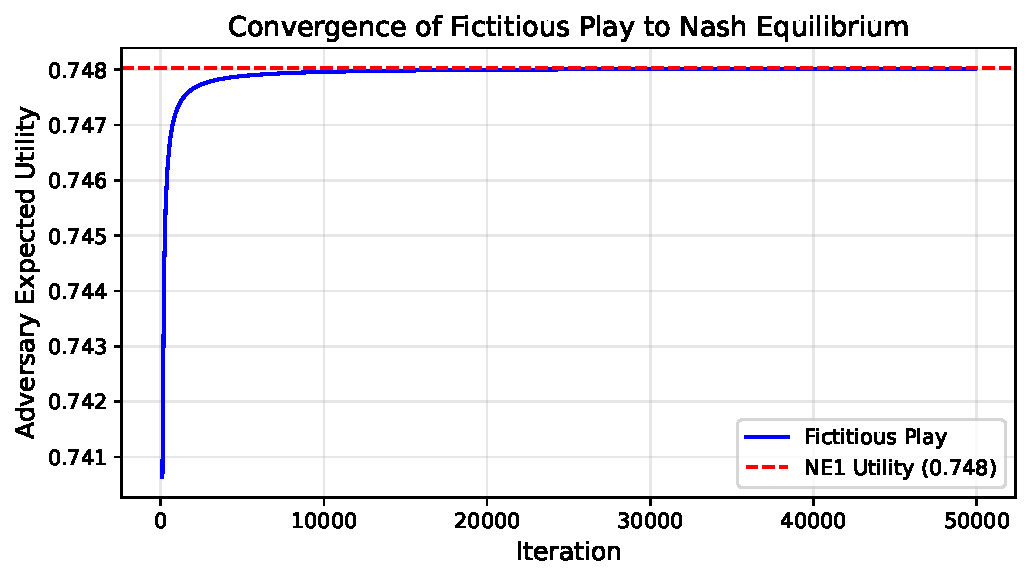
\includegraphics[width=0.6\textwidth]{figures/fictitious_play_convergence.pdf}
    \caption{Fictitious play convergence over 50,000 iterations. The adversary's expected utility converges to NE1 (adversary utility 0.748), validating the equilibrium computation and confirming that myopic best-response dynamics reach the pure-strategy equilibrium where backdoor attacks face an undefended server.}
    \label{fig:convergence}
\end{figure}

\subsection{Impact of Data Heterogeneity}

We sweep across Dirichlet $\alpha \in \{0.1, 0.3, 1.0, 10.0\}$ and adversarial fractions $f \in \{0.1, 0.2, 0.4\}$ to study how equilibrium strategies shift with the operating environment (Figure~\ref{fig:sweep}).

\begin{figure}[t]
    \centering
    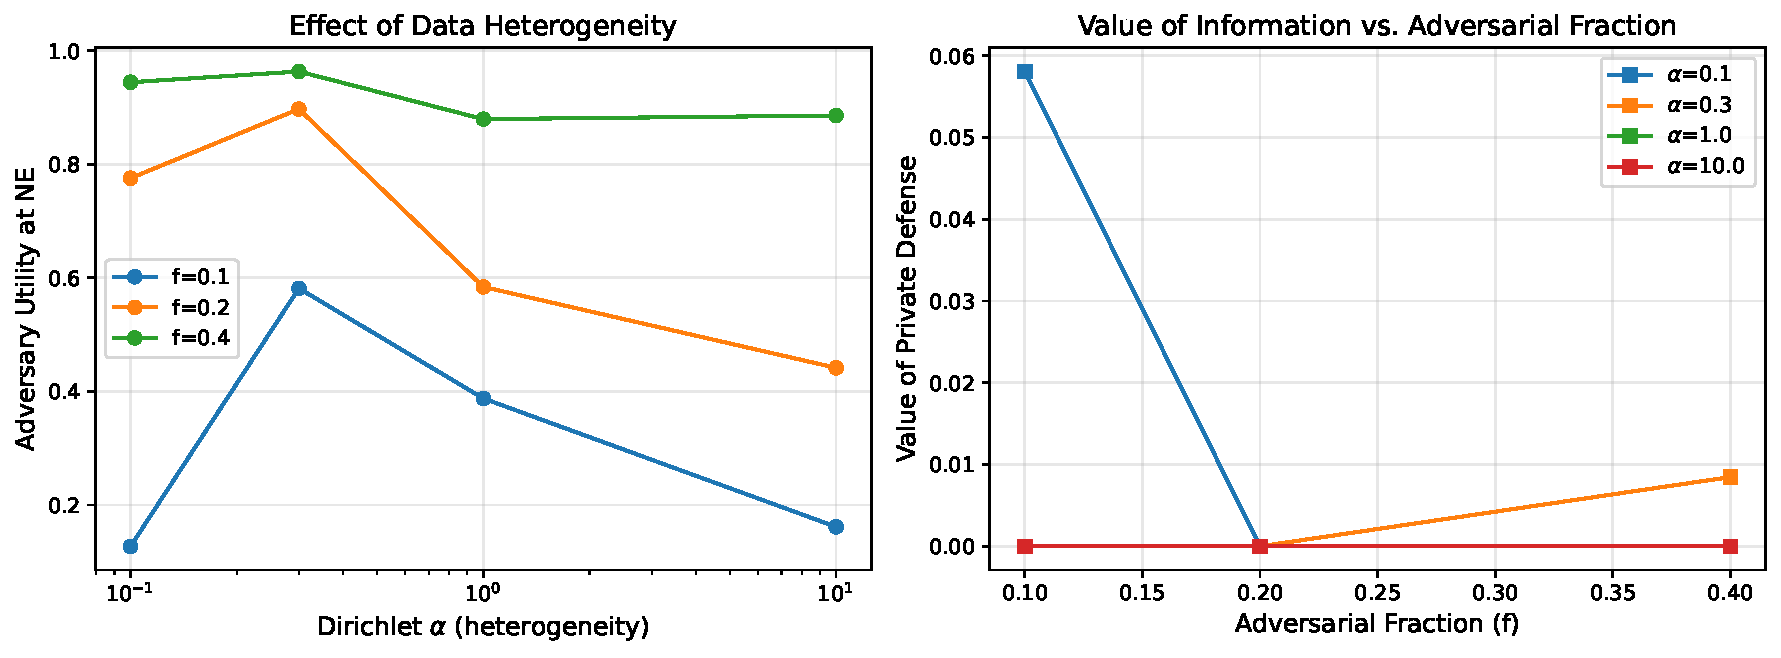
\includegraphics[width=\textwidth]{figures/heterogeneity_sweep.pdf}
    \caption{Left: Adversary equilibrium utility vs.\ data heterogeneity ($\alpha$) for different adversarial fractions. Right: Value of Private Defense vs.\ adversarial fraction for different heterogeneity levels. Adversary equilibrium utility is non-monotone in $\alpha$: at low adversarial fractions ($f=0.1$), moderate non-IID ($\alpha=0.3$) maximizes attack effectiveness, while at higher fractions ($f=0.4$), lower $\alpha$ consistently helps the adversary. Higher $f$ increases both adversary utility and the value of defense secrecy.}
    \label{fig:sweep}
\end{figure}

\subsection{Discussion}

Our experimental findings support the theoretical predictions.

\begin{table}[t]
\caption{Adversary utility under different information structures. The full-information baseline $U_A^{\text{FI}} = 0.906$ is the adversary's payoff from model scaling against Norm Clipping---the highest entry in the payoff matrix (Table~\ref{tab:adv_payoff}). VoPD (Eq.~\ref{eq:vopd}) quantifies how much the adversary would gain from observing the defense each round.}
\label{tab:vopd}
\centering
\begin{tabular}{lcc}
\toprule
\textbf{Scenario} & \textbf{Adversary Utility} & \textbf{Server Utility} \\
\midrule
Full information (adversary knows defense; plays best response) & 0.906 & -- \\
Stackelberg (server commits to FedAvg; adversary observes) & 0.748 & 0.782 \\
Bayes-Nash (NE3: server randomizes; defense private) & 0.748 & 0.778 \\
\midrule
\textbf{Value of Private Defense (VoPD)} & \multicolumn{2}{c}{\textbf{0.065}} \\
\bottomrule
\end{tabular}
\end{table}

\begin{enumerate}
    \item \textbf{Non-trivial mixed strategies} (Theorem 2): NE3 in Table~\ref{tab:equilibria} is the unique mixed-strategy equilibrium. The server randomizes between FedAvg (59\%) and Norm Clipping (41\%) to prevent the adversary from exploiting NormClip's vulnerability to model scaling (ASR~$= 0.94$). The adversary, unable to observe which defense is active, plays backdoor pixel---which achieves ASR~$\approx 0.77$ against both FedAvg and NormClip.
    \item \textbf{Positive VoPD} (Theorem 3): In NE3, VoPD~$= 0.065$ (Table~\ref{tab:vopd})---the adversary would gain $0.065$ additional expected utility (${\approx}9\%$ of its BNE utility of 0.748) if it could observe the defense each round. An adversary that observed NormClip (41\% of rounds) would switch to model scaling (ASR~$= 0.94$); the server's randomization prevents this.
    \item \textbf{Defense cost matters}: Krum imposes severe accuracy costs (51\% under no attack vs.\ 80\% for FedAvg) and is therefore absent from all equilibria. NE3's server mix (FedAvg + NormClip) maintains ${\geq}74\%$ clean accuracy while keeping the adversary uncertain about whether scaling or backdoor defenses are active.
    \item \textbf{Model scaling's double vulnerability}: Model scaling achieves ASR~$= 0.94$ against NormClip but is effectively suppressed by Multi-Krum (ASR~$= 0.57$) and nearly eliminated by Krum (ASR~$= 0.06$). This non-dominance across defenses is what sustains the mixed-strategy server equilibrium.
\end{enumerate}

\textbf{Operational interpretation of VoPD.} In NE3, the server deploys NormClip in 41\% of rounds. A full-information adversary observing NormClip would switch from backdoor pixel (ASR~$= 0.77$) to model scaling (ASR~$= 0.94$), gaining $(0.94 - 0.77) \times 0.41 \approx 0.070$ additional utility---consistent with the computed VoPD of 0.065 (the small difference reflects cost-weight adjustments in the utility function). Operationally: over 100 production rounds, private defense prevents approximately 7 additional successful attacks that a full-information adversary would achieve by opportunistically switching to model scaling on NormClip rounds.

\textbf{VoPD without Norm Clipping.} The VoPD arises specifically because NormClip is the defense most vulnerable to model scaling (ASR~$= 0.94$, the highest entry in the payoff matrix). One might ask whether VoPD collapses if NormClip is excluded from the server's strategy space. We re-run the game analysis on the existing payoff matrices with NormClip removed ($|\SD| = 6$). The result: the server's mixed-strategy equilibrium shifts to FedAvg (75\%) + Trimmed Mean (25\%), and VoPD rises to 0.083. This confirms that VoPD is a structural property of the defense landscape---the presence of defenses with complementary vulnerability profiles---rather than an artifact of NormClip in particular. Even without NormClip, the adversary benefits from knowing which of the remaining defenses is deployed, and the server benefits from keeping that choice private.

\section{Related Work}
\label{sec:related}

\textbf{Data Poisoning in FL.} \citet{chen2017targeted} introduced backdoor attacks via data poisoning. \citet{bagdasaryan2020backdoor} demonstrated model replacement attacks in FL, showing that a single malicious participant can substitute the global model. \citet{wang2020attack} showed edge-case backdoors exploit the tail of the data distribution and bypass many defenses. \citet{xie2019dba} proposed distributed backdoor attacks that decompose triggers across malicious clients to evade detection. A common thread in these works is the assumption that the adversary has full knowledge of the defense---our work relaxes this assumption.

\textbf{Defenses.} \citet{pillutla2019robust} proposed geometric median-based robust aggregation (RFA). \citet{sun2019can} studied norm clipping and argued that backdoor attacks can be mitigated by bounding update magnitudes. Krum and related methods~\citep{blanchard2017machine} select updates based on inter-client distances, providing Byzantine fault tolerance. Despite these defenses, \citet{bhagoji2019analyzing} showed that adaptive attackers with knowledge of the defense can still succeed---motivating our study of the information-asymmetric setting. \citet{kairouz2019advances} provide a comprehensive survey of open problems in FL including robustness.

\textbf{Game Theory in Adversarial ML.} Security games~\citep{tambe2011security} model defender-attacker interactions in physical security using Stackelberg formulations. These have been extended to adversarial machine learning, where attackers and defenders reason about evasion and detection strategies. However, prior game-theoretic treatments of ML security typically assume complete information or focus on evasion attacks rather than poisoning in distributed settings. Our work is distinguished by: (i) modeling the FL-specific structure where defense is an aggregation rule with measurable accuracy costs, (ii) using incomplete information (Bayesian games) rather than the standard Stackelberg assumption, and (iii) empirically grounding the payoff matrices through actual FL training rather than assuming parametric utility forms.

\textbf{Robust Aggregation Under Heterogeneity.} A key challenge in FL defense is that non-IID data distributions make legitimate client updates appear dissimilar, reducing the effectiveness of distance-based defenses like Krum~\citep{kairouz2019advances}. Our game-theoretic framework explicitly accounts for this interaction between heterogeneity and defense effectiveness through the empirical payoff matrices.

\section{Conclusion}
\label{sec:conclusion}

We have presented a game-theoretic framework for analyzing data poisoning robustness in federated learning under a pragmatic threat model where the server's defense remains private. Our Bayesian game formulation captures the non-trivial tradeoffs facing both the server (defense cost vs.\ protection) and the adversary (attack aggressiveness vs.\ detectability).

Our empirical analysis on CIFAR-10 with 6 attacks and 7 defenses (50 rounds, 3 seeds) reveals concrete strategic guidance:
\begin{itemize}
    \item \textbf{For servers}: Randomizing between FedAvg (${\sim}59\%$) and Norm Clipping (${\sim}41\%$) achieves near-optimal defense while keeping the adversary uncertain. This mixed strategy (NE3) improves server utility to 0.778 vs.\ 0.782 at the pure Stackelberg, while reducing the adversary's expected utility by VoPD~$= 0.065$ relative to a full-information oracle.
    \item \textbf{For adversaries}: Under incomplete information, the rational strategy is pure backdoor pixel---which achieves consistent ASR~${\approx}0.77$ against both defenses in the server's mix, rather than risking model scaling that performs poorly if NormClip is not deployed.
    \item \textbf{For system designers}: The Value of Private Defense (VoPD~$= 0.065$) quantifies the security benefit of keeping aggregation rules confidential---a zero-cost intervention that meaningfully degrades adversary capabilities by preventing exploitation of defense-specific weaknesses.
\end{itemize}

\textbf{Limitations.} Our analysis considers a static one-shot game with discrete strategy spaces. Our 50-round FL training achieves $\sim$80\% clean accuracy on CIFAR-10 with 10 clients, though longer training would further increase accuracy and may shift equilibrium utilities. Real interactions may involve repeated play where the adversary learns about the defense over time. The reduced strategy set in the heterogeneity sweep (3 attacks $\times$ 3 defenses) may miss equilibria only visible with the full strategy space. Results are averaged over 3 random seeds with 50 communication rounds; standard deviations are reported in Table~\ref{tab:accuracy}.

\textbf{Future work.} Extending to repeated games with learning dynamics, continuous strategy spaces (e.g., parameterized clipping thresholds), coalition formation among adversaries, and validation on larger-scale models and datasets.

\bibliographystyle{abbrvnat}
\bibliography{references}

\appendix
\section{Full Empirical Payoff Matrices}
\label{app:payoff}

Tables~\ref{tab:adv_payoff} and~\ref{tab:srv_payoff} report the full $6 \times 7$ adversary and server payoff matrices used to compute the Nash equilibria in Section~\ref{sec:experiments}. Adversary payoffs follow Eq.~\ref{eq:adv_utility} with $\lambda_a = 0.1$; server payoffs follow Eq.~\ref{eq:server_utility} with $\lambda_c = 0.1$, $\lambda_f = 0.05$. All values are means over 3 independent seeds ($\alpha=0.5$, $f=0.2$, 50 rounds).

\begin{table}[h]
\caption{Adversary payoff matrix $U_A(a,d)$ (mean over 3 seeds, 50 rounds).}
\label{tab:adv_payoff}
\centering
\small
\begin{tabular}{l|rrrrrrr}
\toprule
 & FedAvg & Krum & M-Krum & TrMean & Median & NClip & RFA \\
\midrule
No attack      &  0.000 &  0.000 &  0.000 &  0.000 &  0.000 &  0.000 &  0.000 \\
Label flip     & -0.010 & -0.010 & -0.010 & -0.010 & -0.010 & -0.010 & -0.010 \\
Backdoor pixel &  0.748 &  0.563 &  0.763 &  0.514 &  0.357 &  0.748 &  0.799 \\
Edge-case      & -0.015 & -0.015 & -0.015 & -0.015 & -0.015 & -0.015 & -0.015 \\
Model scaling  &  0.637 &  0.031 &  0.545 &  0.843 &  0.420 &  0.906 &  0.840 \\
DBA            & -0.003 &  0.043 & -0.003 & -0.001 & -0.003 & -0.003 & -0.001 \\
\bottomrule
\end{tabular}
\end{table}

\begin{table}[h]
\caption{Server payoff matrix $U_D(a,d)$ (mean over 3 seeds, 50 rounds).}
\label{tab:srv_payoff}
\centering
\small
\begin{tabular}{l|rrrrrrr}
\toprule
 & FedAvg & Krum & M-Krum & TrMean & Median & NClip & RFA \\
\midrule
No attack      & 0.783 & 0.480 & 0.781 & 0.765 & 0.750 & 0.780 & 0.762 \\
Label flip     & 0.772 & 0.452 & 0.774 & 0.757 & 0.745 & 0.769 & 0.758 \\
Backdoor pixel & 0.782 & 0.453 & 0.774 & 0.760 & 0.747 & 0.779 & 0.758 \\
Edge-case      & 0.777 & 0.467 & 0.773 & 0.758 & 0.755 & 0.774 & 0.756 \\
Model scaling  & 0.095 & 0.544 & 0.127 & 0.733 & 0.752 & 0.714 & 0.760 \\
DBA            & 0.780 & 0.538 & 0.772 & 0.760 & 0.745 & 0.777 & 0.755 \\
\bottomrule
\end{tabular}
\end{table}

\section{Lambda Sensitivity Analysis}
\label{app:lambda}

Table~\ref{tab:lambda} reports Nash equilibria and VoPD under $\pm 50\%$ perturbations of the cost weights, computed by re-running game analysis on the existing payoff results without re-training.

\begin{table}[h]
\caption{Sensitivity of VoPD and equilibrium support to cost weight perturbations (50-round 3-seed payoffs). Baseline: $\lambda_c=0.1$, $\lambda_f=0.05$, $\lambda_a=0.1$.}
\label{tab:lambda}
\centering
\small
\begin{tabular}{ccc|c|ll}
\toprule
$\lambda_c$ & $\lambda_f$ & $\lambda_a$ & VoPD & Adversary & Server \\
\midrule
0.10 & 0.05 & 0.10 & 0.065 & Pixel (100\%) & FedAvg (59\%) + NClip (41\%) \\
0.05 & 0.05 & 0.10 & 0.065 & Pixel (100\%) & FedAvg (59\%) + NClip (41\%) \\
0.15 & 0.05 & 0.10 & 0.065 & Pixel (99\%)  & FedAvg (59\%) + NClip (41\%) \\
0.10 & 0.025 & 0.10 & 0.065 & Pixel (100\%) & FedAvg (59\%) + NClip (41\%) \\
0.10 & 0.075 & 0.10 & 0.065 & Pixel (100\%) & FedAvg (59\%) + NClip (41\%) \\
0.10 & 0.05 & 0.05 & 0.064 & Pixel (100\%) & FedAvg (61\%) + NClip (39\%) \\
0.10 & 0.05 & 0.15 & 0.066 & Pixel (100\%) & FedAvg (57\%) + NClip (43\%) \\
\bottomrule
\end{tabular}
\end{table}

VoPD is extremely robust: it ranges only from 0.064 to 0.066 across all $\pm 50\%$ perturbations of the three cost weights. The adversary equilibrium support (pure backdoor pixel) and server equilibrium support (FedAvg + NormClip) are qualitatively identical in all configurations; only the FedAvg/NClip mixing ratio shifts by ${\leq}4$ percentage points. These results confirm that the mixed-strategy equilibrium structure and positive VoPD are intrinsic properties of the payoff landscape, not artifacts of the cost parameterization.

\end{document}
